%--------------------------------------------------------------------------------------------------
% 
\chapter{Background}
\label{ch:background}
%--------------------------------------------------------------------------------------------------
Recently, transformer-based models have emerged as the leading performers in multi-label text classification (MLTC), as highlighted by ~\textcite{tarekegn2024deeplearningmultilabellearning}. 
Despite some models achieving high performance without the use of pre-trained language models, as noted by ~\textcite{duan2022fusiontwostream, liu2022cnle}, methods utilizing language pretraining, such as those discussed by~\textcite{yarullin2020bertforseq, fallah2023exploitinglabeldependencies, li2024kenet}, consistently outperform others. 
Most of the revised methods use these models to obtain a dense document representation, a cornerstone of MLTC.
A significant challenge with these pre-trained models is their limitation on text length, which impacts up to 50\% of the instances in our dataset, as illustrated in Figure~\ref{fig:tokens_hist}.

\begin{figure}[h!]
  \centering
  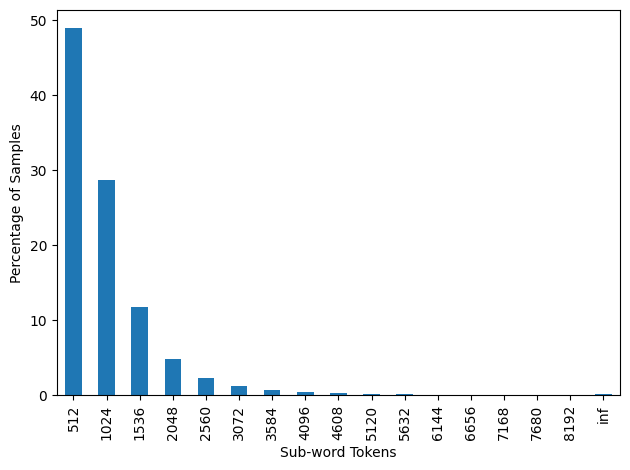
\includegraphics[width=0.6\textwidth]{figures/tokens_hist.png}
  \caption{The distribution of \textit{SentencePiece} sub-word tokens in the $NewsMon$ dataset.}
  \label{fig:tokens_hist}
\end{figure}

Transitioning from standard multi-label text classification to large-scale scenarios shifts the evaluation metrics used, complicating the comparison of different approaches. 
Precision, recall, and F1-score metrics are standard in a typical multi-label setting. 
However, as the scale increases and datasets grow more complex with numerous labels, these metrics might not adequately capture performance nuances.

Extreme and Large-scale classification often incorporates metrics like mean average precision, nDCG (Normalized Discounted Cumulative Gain), and precision at K, considering the ranking of predictions and the relevance of top K labels. 
These metrics are sensitive to the order of labels and the depth of relevance, which are less emphasized in smaller-scale settings.
This metric shift reflects the increased complexity and different priorities in large-scale systems, such as the importance of retrieving the most relevant labels from a vast set. 
% Co-attention network with label embedding for text classification - Co-attention Network with Label Embedding (CNLE)
% Exploiting Label Dependencies for Multi-Label Document Classification Using Transformers - Loss Function adaptation
% Kenet: Knowledge-Enhanced DOC-Label Attention Network for Multi-Label Text Classification

To address this and other challenges, this chapter will first outline the evaluation metrics commonly used in MLTC, focusing on those developed for large-scale multi-label research~\parencite{bhatia2016extremerepo} originating from the field of Information Retrieval (IR)~\parencite{manning2008}. 
Subsequently, we will delve into methods designed to manage text truncation issues inherent in pre-trained language models. 
Finally, we will explore advanced techniques from the most effective MLTC approaches that could potentially refine our methodology and improve performance.

\section{Evaluation Metrics}
Following the work of ~\textcite{tsoumakas2010, madjarov2012, tarekegn2024deeplearningmultilabellearning} and many more, we can observe that all of the well-known classification metrics are used for MLTC research.
While micro averaged $F_1\mhyphen score$ and a $Hamming\mhyphen Loss$ are the most popular in MLTC, they are usually not considered in extreme multi-label text classification (XMTC) research.
In the case of XMTC, the rank-based IR metrics are considered~\parencite{manning2008, bhatia2016extremerepo, chalkidis-etal-2019-large, you2019attentionxmllabeltreebasedattentionaware, chang2020tamingpretrainedtransformersextreme, zhang2023longtailed}.
Therefore, we present three categories of metrics:
\begin{itemize}\itemsep=0pt
    \item Example-based metrics, namely $Hamming\mhyphen Loss$ and $Accuracy$, to assess the differences between the actual and predicted label sets across all instances.
    \item Label-based metrics, including $Precision$, $Recall$, and $F_1\mhyphen score$, to examine performance averaged across all labels.
    \item Rank-based metrics, including $P@K$, $R@K$, $R-precision@K$, and $nDCG@K$
\end{itemize}

In this section, we use $N$ for the number of instances, $L$ for the number of labels, $y_i$ for an individual example label set, and $\hat{y_i}$ for the predicted example label set.

\subsection{Example-based metrics}
For the example-based evaluation, we usually consider
\begin{itemize}
  \item Subset accuracy:
    \begin{equation}
      Accuracy = \frac{1}{N}\sum_{i=1}^{N}I( y_i = \hat{y_i})
    \end{equation}
    where  $I(true) = 1$ and $I(false) = 0$
  \item Hamming loss:
    \begin{equation}
      Hamming\mhyphen Loss = \frac{1}{N \cdot L}\sum_{i=1}^{N}\sum_{j=1}^{L}{xor(y_{i_j},\hat{y_{i_j}})}
    \end{equation}
\end{itemize}
Contrary to Subset accuracy, a Hamming loss closer to 0 means a better score.
\begin{table}[htb]
    \caption{Example $Hamming\mhyphen Loss$ calculation: $\frac{5}{4 \cdot 5} = 0.25$ where each row contains a target $y_i$ followed by a prediction $\hat{y_i}$ vector with five label values with five wrong predictions in total.}
	\label{tab:hamming}
	\centering
    \begin{tabular}{lll}
        \hline
        &$y_i$&$\hat{y_i}$\\
        \hline
        $x_1$&$[1, 0, 1, 1, 0]$&$[1, 0, 1, \textcolor{red}{0}, \textcolor{red}{1}]$\\
        $x_2$&$[0, 1, 1, 0, 0]$&$[0, 1, 1, \textcolor{red}{1}, 1]$\\
        $x_3$&$[0, 0, 0, 1, 0]$&$[0, 0, \textcolor{red}{1}, 1, \textcolor{red}{1}]$\\
        $x_4$&$[1, 1, 0, 1, 0]$&$[1, 1, 0, 1, 0]$\\
        \hline
    \end{tabular}
\end{table}

With a large label set characterized by a long-tail distribution and minimal label density, both Subset accuracy and Hamming loss metrics tend to be very small.
Subset Accuracy tends to be small because such datasets usually have high label diversity versus cardinality; hence, it is hard to predict rare combinations exactly.
Hamming loss is typically very low, which is a desired property. Still, it is low due to the small label cardinality relative to the total number of labels, even when the model performs poorly.

\subsection{Label-based metrics}
For the label-based evaluation, we define:
\begin{itemize}
  \item Micro-averaged Precision and Recall:
    \begin{equation}
      Precision_{micro} = \frac{\sum_{i=1}^{L} TP_i}{\sum_{i=1}^{L} (TP_i + FP_i)}
    \end{equation}
    \begin{equation}
      Recall_{micro} = \frac{\sum_{i=1}^{L} TP_i}{\sum_{i=1}^{L} (TP_i + FN_i)}
    \end{equation}
  \item Macro-averaged Precision and Recall:
    \begin{equation}
      Precision_{macro} = \frac{1}{L}\sum_{i=1}^{L}\frac{TP_i}{TP_i + FP_i}
    \end{equation}
    \begin{equation}
      Recall_{macro} = \frac{1}{L}\sum_{i=1}^{L}\frac{TP_i}{TP_i + FN_i}
    \end{equation}
\end{itemize}
given that:
\begin{itemize}\itemsep=0pt
  \item False Positives (FP): a class or label predicted but not present in the test.
  \item False Negatives (FN): a class or label is present in the test but missing in our prediction.
  \item True Positives (TP): a class or label that is correctly predicted.
  \item True Negatives (TN): a class or label that is correctly not predicted and not present in the test.
\end{itemize}
Precision measures the accuracy of positive predictions, and Recall (also known as sensitivity) measures a classifier's ability to find all relevant instances in a dataset.
In both cases, the harmonic mean of precision and recall, the $F_1\mhyphen score$, can be computed as follows:
\begin{equation}
  F_1\mhyphen score = 2  \cdot \frac{Precision \cdot Recall}{Precision +  Recall}
\end{equation}
% Micro-averaging is more widely used than macro-averaging for MTLC model evaluation. Hmnn

\subsection{Ranking-based metrics}
Common evaluation measures for Large-scale Multi-Label Text Classification (LMTC) include precision (P@K) and recall (R@K) for the top K predicted labels, averaged over test samples:

\begin{equation}
P@K = \frac{1}{N} \sum_{i=1}^N \frac{S_i(K)}{K}
\end{equation}
\begin{equation}
R@K = \frac{1}{N} \sum_{i=1}^N \frac{S_i(K)}{R_i}
\end{equation}

where $K$ is the number of labels to be selected per instance, $N$ is the total number of test instances, $S_i(K)$ is the number of correct labels among those ranked as top $K$ for the i-th instance, and $R_i$ is the number of gold labels for each instance.
Although these measures are widely used in LMTC, \textcite{chalkidis-etal-2019-large} questions their appropriateness for the following reasons:
\begin{itemize}
    \item $R@K$ leads to excessive penalization when instances have more than K gold labels. 
    For example, evaluating at $K = 1$ for a single document with five gold labels returns $R@1 = 0.20$ if the system returns a correct label. 
    The system is penalized even though it cannot return more than one label.
    \item $P@K$ does the same for instances with fewer than $K$ gold labels. 
    For example, evaluating at $K = 5$ for a single document with a single gold label returns $P@1 = 0.20$.
\end{itemize}

Both measures tend to overestimate or underestimate performance on documents where the number of gold labels significantly deviates from $K$.
Due to these limitations, these metrics fail to accurately identify the most effective methods.

Given the issues mentioned, \textcite{chalkidis-etal-2019-large} argues that $R\mhyphen Precision@K$ and $nDCG@K$ offer a more informative and equitable evaluation. These measures adapt to the actual number of gold labels per instance, providing a more accurate performance assessment regardless of whether instances have few or many gold labels. We define the macro-averaged versions of these two measures as follows:
\begin{itemize}
    \item Macro-averaged $R\mhyphen Precision@K$:
        \begin{equation}
        R\mhyphen Precision@K = \frac{1}{N} \sum_{i=1}^N \frac{S_i(K)}{\min(K, R_i)}
        \end{equation}
    This measure is the same as $P@K$ if there are at least $K$ gold labels; otherwise, $K$ is reduced to the number of gold labels.
    For large values of $K$ that tend to exceed the number of gold labels, $R\mhyphen Precision@K$ asymptotically approaches $R@K$.
    \item Macro-averaged $nDCG@K$ (normalized discounted cumulative gain):
        %\begin{equation}
        %nDCG@K = \frac{1}{N} \sum_{i=1}^N \sum_{j=1}^K \frac{2^{S_i(j)} - 1}{log_2(1 + j)}
        %\end{equation}
        In general, we define for each instance:
        \begin{equation}
        DCG@K = \sum_{j=1}^K \frac{gain_j}{discount_j} = \sum_{j=1}^K \frac{2^{S_i(j)} - 1}{log_2(j + 1)}
        \end{equation}
        and normalize it by ideal $IDCG@K$ or maximum $DCG@K$ computed from ground truth labels:
        \begin{equation}
        nDCG@K = \frac{DCG@K}{IDCG@K}
        \end{equation}
        Since there is no ordering of labels in the ground truth in the multi-label case, the equations can be slightly rewritten as:
        \begin{equation}
            \text{DCG}@k := \sum_{l\in {\text{rank}}_k (\hat{\mathbf y})} \frac{\mathbf y_l}{\log(l+1)}
        \end{equation}
        Where $\hat{\mathbf y} \in {\mathbb{R}}^{L}$ is a predicted score vector, $\mathbf y \in \left\lbrace 0, 1 \right\rbrace^L$ is a ground truth label vector, $\text{rank}_k(\mathbf y)$ returns the $k$ largest indices of $y$ ranked in descending order~\parencite{bhatia2016extremerepo}.
        \begin{equation}
            \text{nDCG}@k := \frac{{\text{DCG}}@k}{\sum_{l=1}^{\min(k, \|\mathbf y\|_0)} \frac{1}{\log(l+1)}},
        \end{equation}
        Finally, we define micro-averaged value as:
        \begin{equation}
        nDCG@K = \frac{1}{N} \sum_{i=1}^N nDCG@K_i
        \end{equation}
\end{itemize}

\section{Long Document Representation}
\label{sec:long_doc}

The shift from classifying short to long documents presents significant challenges. BERT~\parencite{devlin2018bert}, RoBERTa~\parencite{liu2019roberta}, XLM-RoBBERTa~\parencite{conneau2019xlmr} and many related models are pre-trained on sequences of up to 512 tokens, which can not be considered a long document. A typical method involves truncating longer documents to the first 512 tokens, enabling the direct use of these pre-trained models. 
However, truncating text can exclude critical information; therefore, we believe this approach is insufficient for long document classification. 
This can negatively affect the classification performance. 
Another significant challenge is the computational and memory overhead associated with the vanilla Transformer architecture's $O(n^2)$ complexity, which prevented using longer contexts before the LLM era.

Early approaches were based on sparse self-attention instead of full-self attention (Longformer; \textcite{beltagy2020longformerlongdocumenttransformer},  and Big Bird; \textcite{zaheer2021bigbird}), dividing long documents into smaller chunks (Hierarchical Transformers; \textcite{pappagari2019hierarchical}), or using only selected sentences from the document that are salient to making the classification decision (CogLTX; \textcite{ding2020cogltx}).

\begin{table}[H]
	\centering
    \resizebox{\textwidth}{!}{%
        \begin{tabular}{lccccccc}
        \hline
        \textbf{Dataset} & \textbf{Type} & \textbf{\# Train} & \textbf{\# Dev} & \textbf{\# Test} & \textbf{\# Labels} & \textbf{\# BERT Tokens} & \textbf{\% Long} \\
        \hline
        Hyperpartisan & binary & 516 & 64 & 65 & 2 & 744.18 ± 677.87 & 53.49 \\
        20NewsGroups & multi-class & 10,182 & 1,132 & 7,332 & 20 & 368.83 ± 778.34 & 11.30 \\
        EURLEX57K & multi-label & 45,000 & 6,000 & 6,000 & 4,271 & 707.99 ± 538.69 & 51.30 \\
        Inverted & multi-label & 10,230 & 1,279 & 1,279 & 227 & 574.31 ± 659.56 & 38.76 \\
        Book Summary & multi-label & 5,115 & 639 & 639 & 227 & 1,148.62 ± 933.97 & 75.54 \\
        \hline
        \end{tabular}
    }
\caption{Statistics on the datasets. \# BERT Tokens refers to the average token count obtained via the tokenizer of the BERT base model (uncased). \% Long refers to the percentage of documents with more than 512 BERT tokens~\parencite{park2022efficient}.}
\label{tab:park_dataset}
\end{table}

\begin{table}[H]
	\centering
    \resizebox{\textwidth}{!}{%
        \begin{tabular}{lcccccc}
        \hline
        \rule{0pt}{4ex} \textbf{Model} & \textbf{Hyperpartisan} & \textbf{20NewsGroups} & \textbf{EURLEX} & \rule[-2ex]{0pt}{0pt} \parbox[c]{2cm}{\textbf{Inverted\newline EURLEX}} & \parbox[c]{2cm}{\textbf{Book\newline Summary}} & \parbox[c]{2cm}{\textbf{Paired\newline Summary}} \\
        \hline
        BERT & 88.00 & \underline{86.09} & \underline{66.76} & 62.88 & 60.56 & 52.23 \\
        BERT+TextRank & 85.63 & 85.55 & 66.56 & \underline{64.22} & 61.76 & 56.24 \\
        BERT+Random & 83.50 & \textbf{86.18} & \textbf{67.03} & \textbf{64.31} & \textbf{62.34} & 56.77 \\
        Longformer & \textbf{93.17} & 85.50 & 44.66 & 47.00 & 59.00 & \textbf{58.85} \\
        ToBERT & 86.50 & -- & 61.85 & 59.50 & 61.38 & \underline{58.17} \\
        CogLTX & \underline{91.91} & 86.07 & 61.95 & 63.00 & 60.71 & 55.74 \\
        \hline
        \end{tabular}
    }
\caption{Performance metrics evaluated on long documents in the test set for all datasets. The average accuracy (\%) over five runs is reported for Hyperpartisan and 20NewsGroups, while the average micro-F1 (\%) is used for the other datasets. The highest value per column is in bold, and the second highest value is underlined~\parencite{park2022efficient}.}
\label{tab:park_longdoc}
\end{table}

\textcite{park2022efficient} argues that the effectiveness of various models remains ambiguous due to the absence of a unified consensus on benchmark datasets and established baselines. 
Often, new variants of efficient Transformers are only compared against a BERT/RoBERTa baseline, with limited comparisons to other Transformer models designed explicitly for the task~\parencite{beltagy2020longformerlongdocumenttransformer, zaheer2021bigbird}.
Conversely, models tailored for long document classification typically focus solely on comparing state-of-the-art models for specific datasets. 
They frequently overlook the inclusion of a BERT/RoBERTa baseline or comparisons~\parencite{pappagari2019hierarchical, ding2020cogltx}.



While \textcite{dai2022revisitingtransformer} research suggests that using Longformer or Hierarchical Transformers enhances performance in long document classification, \textcite{park2022efficient} and \textcite{jaiswal2023breakingtokenbarrierchunking} findings indicate the opposite, in the latter, vanilla BERT with 512 tokens extended random-sentence text block outperformed more advanced models (BERT and BERT-random CLS tokens were concatenated before the classification head, see Table~\ref{tab:park_longdoc}). 
Both studies demonstrate that the effectiveness of these models is highly dependent on the dataset used.
It is worth noting that all experiments were conducted using English-language pre-trained models and datasets.

\section{Extending the Position Encoding}
The development of pre-trained language models has driven innovations in text embedding techniques, including Sentence-BERT~\parencite{reimers-2019-sentence-bert} and SimCSE~\parencite{gao2022simcse}, which refine BERT by fine-tuning on natural language inference (NLI) datasets. 
To push the boundaries of text embedding performance and robustness, advanced methods and models designed for RAG and IR, like E5~\parencite{wang2024textembeddingsweaklysupervisedcontrastive} and BGE~\parencite{xiao2024cpackpackagedresourcesadvance} have been introduced. 
These methods implement a complex multi-stage training approach, beginning with pre-training on billions of weakly supervised text pairs and then fine-tuning on various high-quality labelled datasets. In both stages, contrastive learning plays a crucial role.
The process of contrastive learning involves selecting a random example as an anchor and then choosing positive and negative examples related to the anchor. 
Subsequently, positive examples are drawn closer to the anchor, while negative examples are pushed further away.

In recent years, reasonably sized models with impressive performance from this family have emerged, some even multilingual~\parencite{wang2024multilinguale5textembeddings}. 
However, many of these models are initialized from traditional pre-trained Transformer architectures and inherit their limitations, such as short context windows and, consequently, truncated text.
To address this issue, approaches have been developed to capture broader contexts and more comprehensive document semantics with modifications of positional encoding without the need to train the model from scratch.
\textcite{zhu2024longembedextendingembeddingmodels} provides a comprehensive \textit{LongEmbed} benchmark for both absolute positional and rotary positional encoding modifications to enable context window extension.
\begin{itemize}
    \item \textbf{Absolute Position Encoding (APE)} is the most common positional encoding technique used in models that follow the BERT architecture. In APE-based models, absolute position identifiers are converted into position vectors, which are then added to token embeddings. This combined input is subsequently processed through a series of transformer layers.
    \item \textbf{Rotary Position Encoding (RoPE)} is the most common position encoding strategy used in the era of LLMs, including LLaMA~\parencite{touvron2023llama}, Gemma~\parencite{gemma_2024}, Mistral~\parencite{jiang2023mistral7b}, etc. 
    It encodes position information of tokens with a rotation matrix that naturally incorporates explicit relative position dependency.
\end{itemize}
\textcite{zhu2024longembedextendingembeddingmodels} further categorizes the strategies for managing long input sequences in model processing:
\begin{enumerate}
    \item \textbf{Divide-and-Conquer:} This approach segments long inputs into shorter chunks, processes each individually, and then combines the results. This method is used in the PCW model \parencite{ratner2023parallelcontextwindowslarge}.
    \item \textbf{Position Reorganization:} This technique rearranges position identifiers to enhance the model's ability to handle longer sequences. Examples include SelfExtend \parencite{jin2024llmmaybelonglmselfextend} and DCA \parencite{an2024trainingfreelongcontextscalinglarge}, among others.
    \item \textbf{Position Interpolation:} This involves creating new position embeddings by interpolating between existing ones. Models employing this technique include PI \parencite{chen2023extendingcontextwindowlarge}, NTK \parencite{peng2023ntkaware}, YaRN \parencite{peng2023yarnefficientcontextwindow}, and Resonance RoPE \parencite{wang2024resonanceropeimprovingcontext}.
\end{enumerate}
Extending the Position Encoding allows for a more adequate representation of longer texts, enabling the retrieval system to consider the document as a whole rather than in fragmented parts.
While some of these methods can be used effectively on APE without additional fine-tuning (Parallel Context Windows, Grouped Positions, Recurrent Positions, Linear Position Interpolation), they generally yield better results when fine-tuned~\parencite{zhu2024longembedextendingembeddingmodels}.
There has been a noticeable trend in models designed for information retrieval (IR) that are initialized from large language models (LLMs), moving away from the previously predominant Transformer-Encoders.

\section{Recent MLTC and XMTC approaches}
In this section, we explore some of the recent state-of-the-art (SOTA) approaches in both Multi-Label Text Classification (MLTC) and Extreme Multi-Label Text Classification (XMTC), as datasets with similar sizes and properties appear in the research of both. 
Reviewing these methodologies, we aim to gain insights that could refine our approach.

We can split the document classification model into two parts: a document encoder that creates a dense document representation and a classifier that predicts one or multiple labels based on the encoded representation~\parencite{dai2022revisitingtransformer}. 

Multiple data labels often indicate relationships between different categories, leading recent methods to commonly address the issue of Label Dependency. 
In terms of modelling these dependencies, learning approaches are categorized into first-order (each label treated independently), second-order (modelling interactions between pairs of labels), and higher-order (addressing interactions among more than two labels simultaneously)~\parencite{tarekegn2024deeplearningmultilabellearning}.

Binary cross-entropy loss (BCE; \textcite{bengio2013bce}), when paired with a sigmoid activation function, is widely used in machine learning for addressing multi-label classification problems and can be considered a baseline loss function. 
With BCE, each label is considered an independent binary prediction.
The main challenge with BCE arises from the imbalance in label distribution and the complex dependencies among labels, which have inspired numerous studies on loss function design.
Focal loss (FL), introduced by \textcite{lin2017focal}, assigns greater weight to instances that are less likely to occur, which is interpreted as "harder to classify." 
Class-Balanced loss (CB), proposed by \textcite{cui2019classbalanced}, implements a re-weighting scheme upon FC based on the effective number of instances per class, reducing redundant information of head classes. 
Distribution-Balanced loss (DB) by \textcite{wu2020distributionbalanced} initially reduces redundant information resulting from label co-occurrence. Then, it incorporates Negative Tolerant Regularization (NTR) to reduce the weight of easy-to-classify negative labels.
Building on this, CB-NTR Loss by \textcite{huang2021balancing} combines the features of CB and NTR to better handle label imbalances and dependencies~\parencite{ma2023pai}.
A similar approach is taken by \textcite{fallah2023exploitinglabeldependencies}, which computes loss regularization term based on the dis-similarity vector - a result of the label co-occurrence matrix and the activations of the output layer of the classification.

In addition to incorporating label co-occurrence and imbalances into the loss function computation, contrastive learning techniques have become popular in some multi-label classification tasks~\parencite{piskorski-etal-2023-semeval-task3}.
For multi-label text classification, these methods often calculate a combined loss that includes both binary cross entropy and contrastive loss~\parencite{reiterhaas2023mcpt, liao2023marseclipse}.
Interestingly, we encountered similar techniques widely used in computer vision~\parencite{zheng-etal-2022-contrastive, tunstall2022efficient} as predominant in learning the dense document representations for IR and RAG systems in the previous Section~\ref{sec:long_doc}.

\begin{figure}[h!]
  \centering
  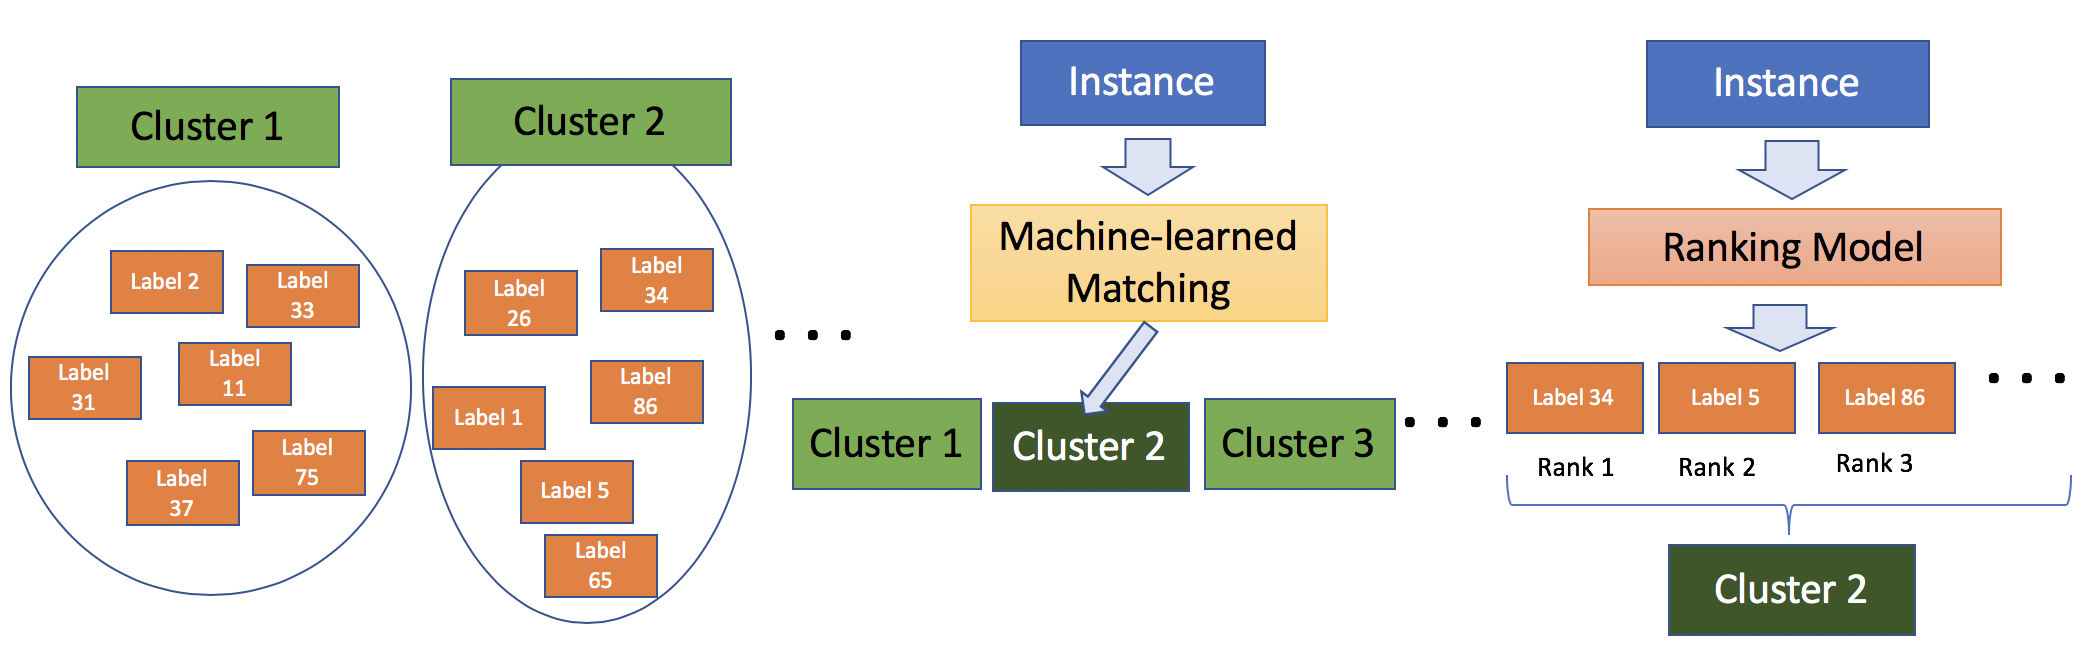
\includegraphics[width=0.9\textwidth]{figures/x-transformer_model.png}
  \caption{The proposed X-Transformer framework. First, Semantic Label Indexing reduces the large output space. Transformers are then fine-tuned on the XMTC sub-problem that maps instances to label clusters. Finally, linear rankers are trained conditionally on the clusters and Transformer’s output to re-rank the labels within the predicted clusters.~\parencite{chang2020tamingpretrainedtransformersextreme}.}
  \label{fig:x_trans_model}
\end{figure}

%TODO: in batch negative sampling popular in XMTC

Another class of approaches integrates label semantics directly into the neural network architecture by combining dense document representations with label representations. 
These methods differ in using either sparse or dense label representations and whether they employ the same or different encoders at various stages for labels and documents.
For example, in the domain of XMLC, sparse label representations are employed alongside Label Semantic Indexing to cluster labels and simplify the classification challenge with a large label count (see Figure\ref{fig:x_trans_model}). 

\begin{figure}[h!]
  \centering
  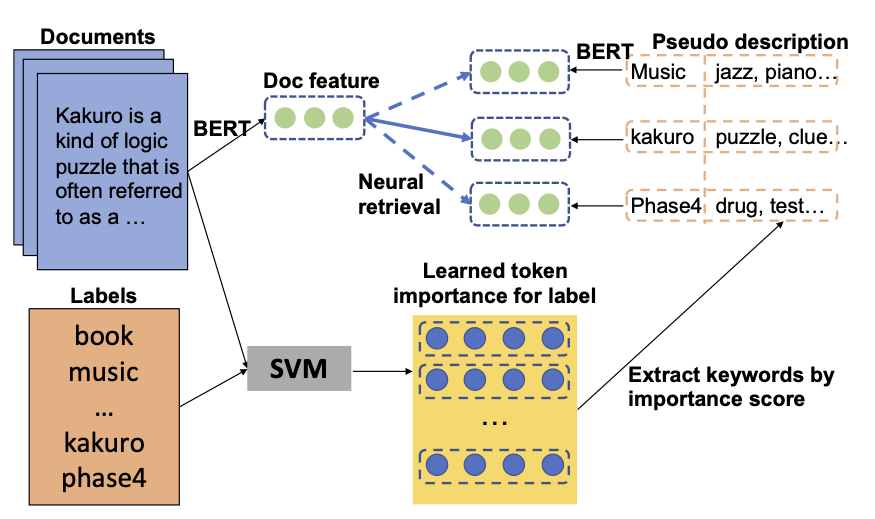
\includegraphics[width=0.5\textwidth]{figures/depl_model_2.png}
  \caption{The proposed DEPL framework. First, a BoW SVM classifier is trained, and top keywords from the label embeddings are extracted according to the importance of the learned token. 
  Then, keywords are concatenated with the original label names to form pseudo descriptions. 
  Finally, a neural retrieval model is leveraged to rank the labels according to semantic matching between document text and label descriptions~\parencite{zhang2023longtailed}.}
  \label{fig:depl_model}
\end{figure}

More recently, another method has improved the prediction of tail labels over the X-Transformer model. 
The DEPL model proposed by \textcite{zhang2023longtailed} uses sparse representations to augment labels with pseudo descriptions, which are then processed by the same encoder as documents. 
The SVM classification model is used to identify and concatenate the most important keywords related to each label, creating pseudo descriptions.
Specifically, they encode all the positive labels of the instances in the batch, add the top negative predictions from the sparse classifier, and include randomly sampled negatives to complete the batch. 
The loss is then calculated based on both positive and retrieved negative values during the training process (see Figure~\ref{fig:depl_model}).
This negative in-batch sampling technique is again similar to how other XMTC models~\parencite{jiang2021lightxmltransformerdynamicnegative} are trained and is inspired by IR models~\parencite{karpukhin2020dense}.

\begin{figure}[h!]
  \centering
  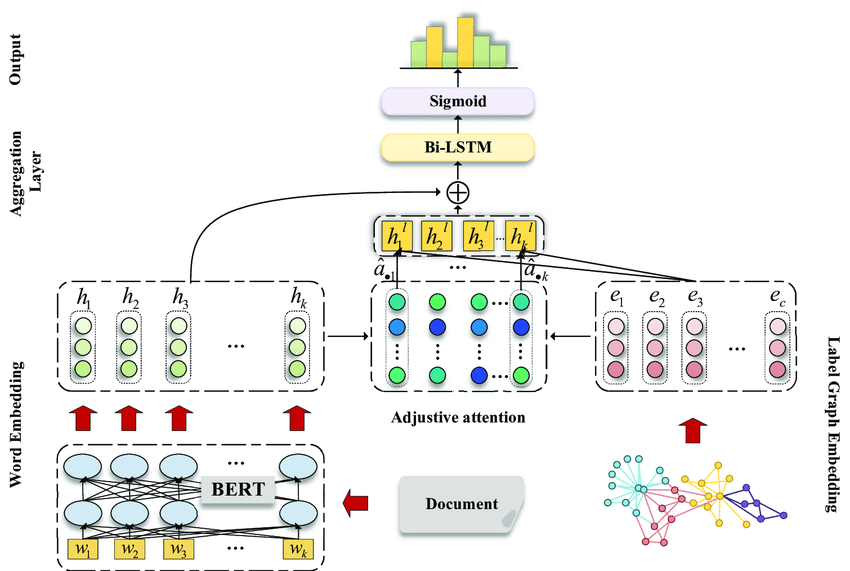
\includegraphics[width=0.6\textwidth]{figures/hbla_model.png}
  \caption{HBLA model~\parencite{cai2020hbla}.}
  \label{fig:hbla_model}
\end{figure}

In the domain of MLTC, the hybrid BERT model that incorporates label semantics via adaptive attention (HBLA), introduced by \textcite{cai2020hbla}, shows an advanced approach to addressing label dependencies. 
HBLA can simultaneously model a document and a label and obtain the hybrid word representation by an innovative adjustive attention mechanism that calculates the semantic relationships between words and labels.
It uses a graph convolutional network to capture label correlations through a label graph constructed from adjacency-based similarity as shown in Figure~\ref{fig:hbla_model}.

\begin{figure}[h!]
  \centering
  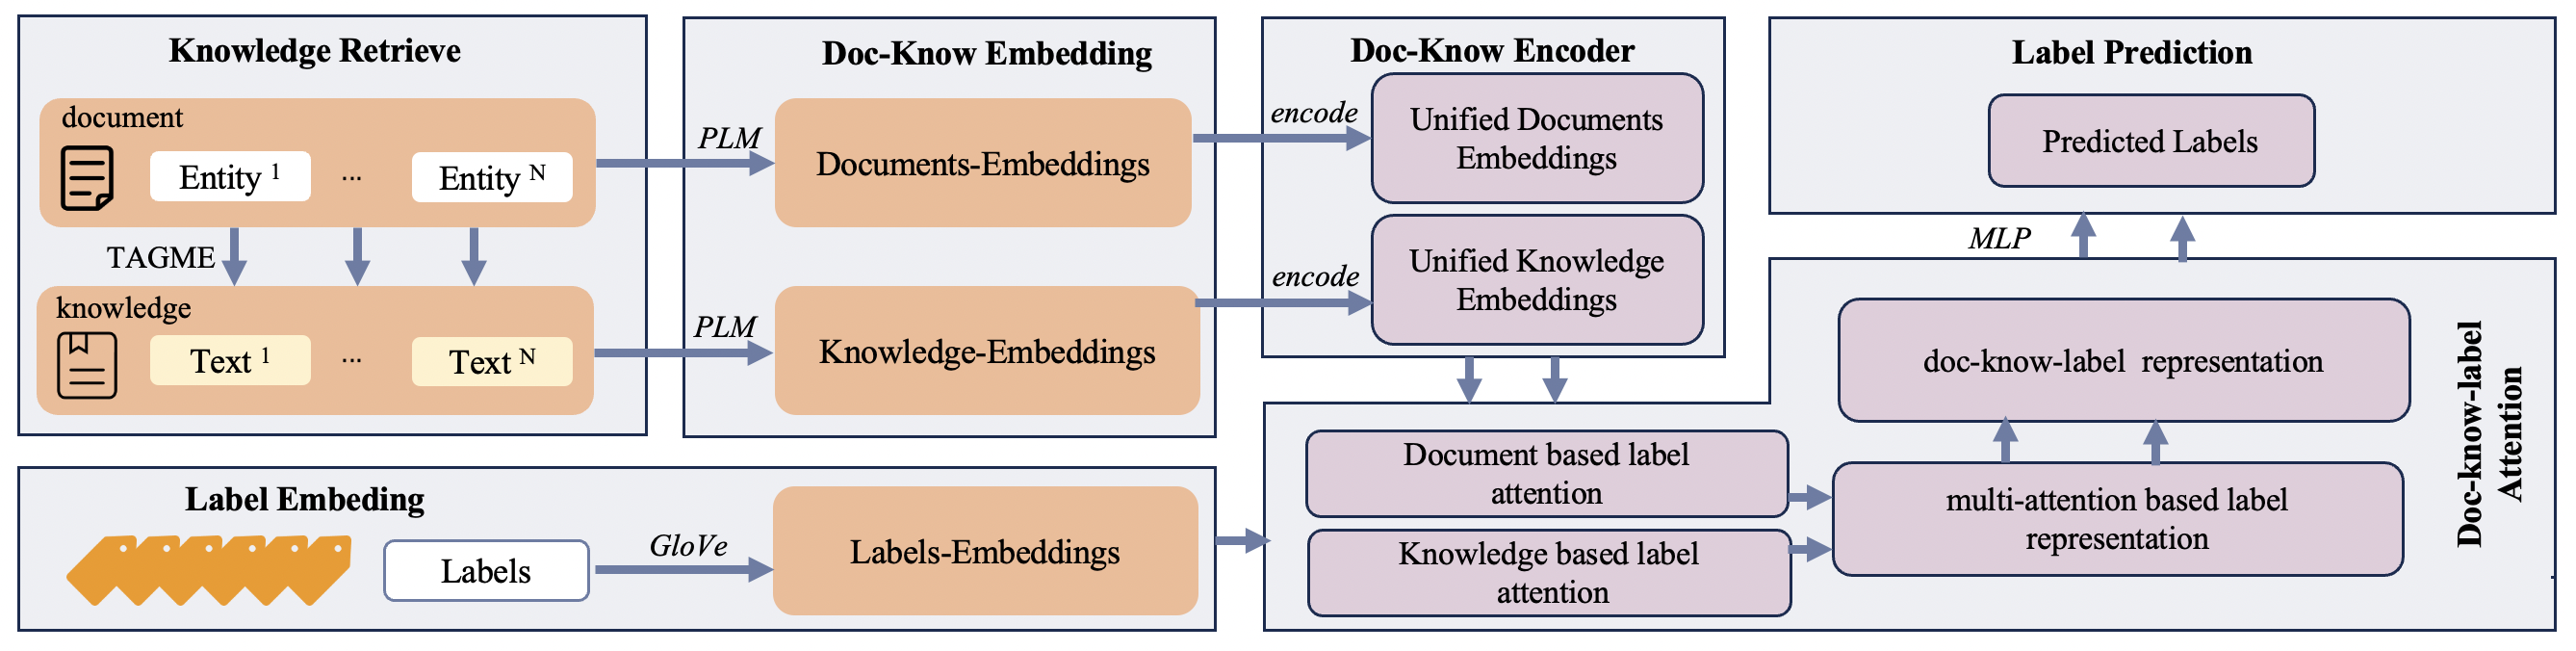
\includegraphics[width=0.9\textwidth]{figures/kenet_model.png}
  \caption{KeNet model~\parencite{li2024kenet}.}
  \label{fig:kenet_model}
\end{figure}

\textcite{li2024kenet} introduced the KeNet model, which demonstrates a retrieval-enhanced approach, utilizing knowledge retrieved from Wikipedia along with document embeddings. 
Both are processed using the same BERT encoder, while label embeddings are created using a GloVe~\parencite{pennington2014glove} encoder. 
These components are integrated through a Document-Knowledge-Label attention mechanism. 
This mechanism combines weighted attention between document-label and knowledge-label and effectively fuses information across documents, external knowledge, and labels to enhance data processing and interpretation.
Both MLTC methods presented above use BCE loss and sigmoid activation function for classification.
